\documentclass[preview]{standalone}

\usepackage{amsmath}
\usepackage{fullpage}
\usepackage{tikz}
\usepackage{hyperref}
\usepackage{stellar}

\hypersetup{
    colorlinks=true,
    linkcolor=black,
    urlcolor=blue,
    pdftitle={Ray-Sphere Intersection},
    pdfpagemode=FullScreen,
}

\begin{document}

\title{Ray-Sphere Intersection}
\id{raysphereintersection}
\genpage

\section{Derivation}

\begin{snippet}{ray-sphere-intersection-illustration}
\begin{center}
	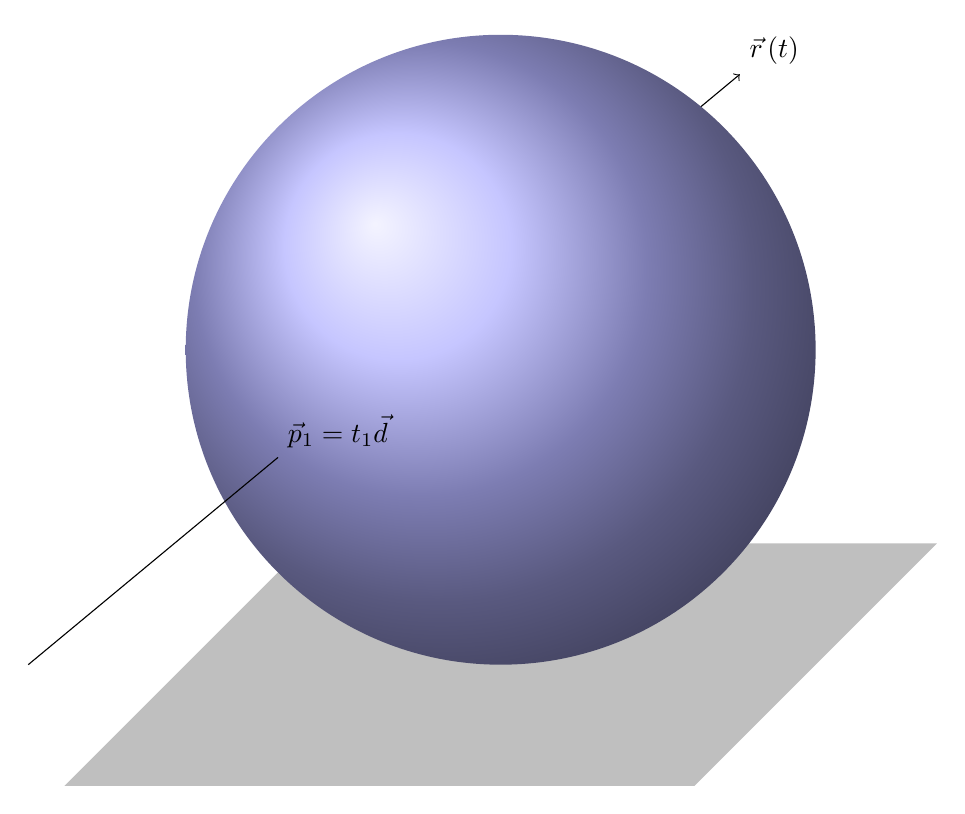
\begin{tikzpicture}[scale=2]
		% values are wrong
		\fill[opacity=0.25] (-2,-2,-2) -- (2,-2,-2) -- (2,-2,2) -- (-2,-2,2) -- cycle;
		\draw [->] (1.49,1.9,2.69) -- (2.87,3.1,3.51) node [above right] {\(\vec{r}\,(t)\)};
		\shade[ball color=blue!30] (0,0,0) circle (2);
		\draw [-] (-3,-2,0) -- (-0.94,-0.21,1.23) node [above right] {\(\vec{p}_1=t_1\vec{d}\)};
	\end{tikzpicture}
\end{center}
\end{snippet}

\begin{snippet}{ray-sphere-intersection-derivation}
We are given:
\begin{itemize}
	\item The ray origin \(\vec{o}\)
	\item The ray direction \(\vec{d}\) such that \(||\vec{d}\,||=1\)
	\item The center of the sphere \(\vec{c}\)
	\item The radius of the sphere \(r\)
\end{itemize}

The position of the ray after travelling \(t\) distance is given by
\[
    \vec{r}\,(t)=\vec{o}+t\vec{d}
\]
    
The equation of the sphere is given by
\[
    {(\vec{p}-\vec{c}\,)}^2=r^2
\]
        
where \(\vec{p}\) is a point on the surface of the sphere.

We want to find the distance \(t\) for which the ray intersects with the surface of the sphere.
\[
    \vec{p}=\vec{o}+t\vec{d}
\]

We substitute the definition of \(\vec{p}\) into the sphere equation.
\begin{align*}
	\Big(\vec{o}+t\vec{d}-\vec{c}\,\Big)\Big(\vec{o}+t\vec{d}-\vec{c}\,\Big)&=r^2\\
	\underbrace{\Big(\vec{d}\cdot\vec{d}\,\Big)}_\text{A}t^2+
	\underbrace{2\vec{d}\,\Big(\vec{o}-\vec{c}\,\Big)}_\text{B}t+
	\underbrace{{\Big(\vec{o}-\vec{c}\,\Big)}^2-r^2}_\text{C}&=0\\
\end{align*}

We can then rewrite the equation as
\[
    At^2+Bt+C=0
\]
    
Using the quadratic formula
\[
    \vec{t}_{1,2}=\frac{-B\pm\sqrt{\Delta}}{2A}
\]

Where \(\Delta=B^2-4AC\)

The points of collision are \(\vec{p}_1=\vec{r}\,(t_1)\) and \(\vec{p}_2=\vec{r}\,(t_2)\).

The points of collision could be 2, 1 or none.
\begin{align*}
	\begin{cases}
		2,\quad\text{if }\Delta<0\\
		1,\quad\text{if }\Delta=0\\
		0,\quad\text{if }\Delta>0
	\end{cases}
\end{align*}

If \(t_1\) or \(t_2\) is negative, the intersects is behind the ray (or camera).

If \(t_1\) or \(t_2\) is \(0\), the collision is the ray or camera itself.

Discard those points if you are rendering.
\end{snippet}

\end{document}